\documentclass[acmsmall,nonacm]{acmart}

\settopmatter{printacmref=false}

\citestyle{acmnumeric}

\usepackage{booktabs}

\usepackage{tabularx}

\usepackage{graphicx}

\usepackage{float}

\title{Citation Priors and Top-K Recall in a Review-Grounded Literature Corpus: A Reproducible Pilot}

\author{Rohit Mahali}

\affiliation{\institution{Indian Institute of Information Technology Allahabad}\city{Prayagraj}\country{India}}

\begin{document}

\begin{abstract}AI-assisted literature curation can reduce search effort while altering which papers appear near the top of a ranked list. The supplied review identifies citation status as a possible source of recall loss and calls for stratified benchmarks, but it provides no executable ranking experiment. This pilot tests a narrow mechanism: adding an explicit citation-count prior to lexical retrieval. We construct a fixed corpus from the 15 works cited by the review, annotate four query-specific relevant sets from its evidence map, and compare BM25, TF-IDF cosine, and BM25 with a min-max normalized log citation prior. On an OpenAlex snapshot retrieved on 17 November 2026, both lexical baselines achieve macro Recall@5 of 0.917 and low-citation Recall@5 of 1.000. The citation-prior system at weight 0.25 achieves 0.804 and 0.750, while mean log1p citations among its top-five results rises from 3.650 for BM25 to 5.640. A weight sensitivity analysis shows the low-citation recall decline emerging at weights of 0.25 and above. These measurements demonstrate a ranking trade-off inside this small, review-derived bibliography. They do not estimate field-wide recall, validate an LLM recommender, or establish language fairness. The frozen metadata, query labels, code, rankings, and outputs are included for inspection and rerun.\end{abstract}

\keywords{literature retrieval, citation bias, recall, BM25, bibliographic metadata, reproducibility}

\maketitle

\section*{1 Introduction}

Literature curation systems discover, rank, screen, and synthesize research records. The supplied narrative review connects these stages to two possible sources of recall loss: citation status and language or corpus coverage \cite{mahali2026review}. Its cited evidence includes work finding that LLM-generated paper references reflect human citation patterns with an even stronger high-citation tendency \cite{algaba2025citation}, and work reporting that paper recommenders prefer papers with greater citation counts \cite{tian2024recommendation}. These findings motivate a focused implementation question about ranking, where the intervention and its effect can be isolated.\par

A citation prior is not inherently harmful. Citations can indicate influence and help locate foundational work. The risk addressed here is narrower: when citation count is added to topical relevance, a paper's existing visibility may influence which candidate records fit into a limited screening budget. The Matthew effect provides a theoretical reason to inspect cumulative visibility \cite{merton1968}, but this pilot does not treat citation count as a measure of quality, correctness, or relevance.\par

The goal is a small controlled study that can run on a local CPU without proprietary models or restricted datasets. We take the 15 works in the review's reference list as a fixed candidate corpus and use four queries grounded in the review's own evidence map. The bibliography makes the experiment tractable and traceable, while also sharply limiting what its recall values mean.\par

The primary question is: for four review-grounded topic queries over the review's 15 cited works, how does adding an OpenAlex citation-count prior to BM25 affect Recall@5 for manually annotated relevant references, especially those in the corpus-relative lowest citation third? We compare BM25 and TF-IDF as lexical baselines with BM25 plus a citation prior. The contribution is a reproducible pilot and a measured account of its ranking behavior, not a new search algorithm or a claim about LLM recommendation quality.\par

\section*{2 Evidence base and study boundary}

The review motivating this study is a narrative review rather than a registered systematic review. It defines recall as relevant records retrieved divided by all relevant records, discusses subgroup recall differences, and explicitly cautions that its cross-study comparison is not a leaderboard because tasks, domains, and protocols differ \cite{mahali2026review}. Its future-work section asks for language- and citation-stratified benchmarks, corpus audits, source provenance, and evaluation of adaptive retrieval.\par

The original source for the citation-bias motivation was checked against the ACL Anthology record for Algaba et al. \cite{algaba2025citation}, which confirms the paper metadata and reports a stronger high-citation bias in recommendations from several LLMs. The arXiv record for Tian et al. \cite{tian2024recommendation} identifies its submission as 31 December 2024 and describes a recommendation experiment in which citation counts, publication date, and team size influenced recommendations. The primary IOS Press record for Ikeguchi et al. \cite{ikeguchi2026language} confirms a separate multilingual screening result: 2,911 English records and 483 non-English abstracts, with sensitivity falling to 0.47-0.54 for some translated inputs while direct multilingual processing ranged from 0.71 to 1.00. This language result motivates the broader review but is not measured in the present experiment.\par

Agarwal et al. \cite{agarwal2025litllms} is also relevant because its TMLR/OpenReview record describes retrieval, reranking, and attribution in literature-review assistance. That work studies a different method and benchmark. We do not claim to reproduce it: this pilot uses only transparent lexical rankers and an explicit metadata prior. Retrieval-augmented generation combines external retrieval with model generation \cite{lewis2020rag}, but no generative component is included here.\par

The corpus is deliberately the review's bibliography rather than a newly searched literature collection. Consequently, a positive label means that the review uses a cited work as evidence for a particular query topic. A missing positive in the top five is a ranking miss within this annotation set. The study cannot count relevant works absent from the bibliography, and its query labels are neither independent screening judgments nor a complete domain benchmark.\par

\section*{3 Corpus, queries, and relevance labels}

The candidate set contains the 15 numbered references in the supplied review. A fetch script resolves works using exact DOI endpoints where a DOI is listed and normalized exact-title matching for title-only lookups. OpenAlex returned a record for each input. The frozen snapshot was retrieved on 17 November 2026 and stores OpenAlex work IDs, DOIs, titles, publication years, language, cited-by counts, and reconstructed abstracts. Fourteen records had an abstract in the returned metadata; R04 did not and is represented by its title only.\par

The query and gold-reference sets were fixed in the protocol before ranking outputs were produced. The labels were derived from the review's Sections 3, 4, 5, 7, and 9 and Table 2. Each query has a direct evidence mapping to the review; the full annotation rationale is stored in the protocol and expanded in data/gold\_labels.csv. The positive set sizes are 3, 4, 5, and 3, respectively. All other records are treated as non-positive for that query, not as universally irrelevant papers.\par

\begin{table}[H]
\caption{Frozen query topics and review-derived relevant records.}
\centering\small
\begin{tabularx}{\linewidth}{XXXX}
\toprule
Query & Topic & Relevant reference IDs & n \\
\midrule
Q1 citation recommendation & Citation status in paper recommendations & R02, R08, R15 & 3 \\
Q2 language bias & Language bias in reviews & R05, R09, R12, R14 & 4 \\
Q3 LLM screening & LLM eligibility screening & R03, R04, R05, R07, R13 & 5 \\
Q4 retrieval and RAG & Retrieval and RAG & R01, R06, R11 & 3 \\
\bottomrule
\end{tabularx}
\end{table}

OpenAlex citation counts are time-varying and record-specific. R06 is identified by its arXiv DOI for the NeurIPS paper; a second OpenAlex record with the same title reports a different count. R01 is represented by an arXiv-indexed OpenAlex record with publication year 2024, while the review cites its TMLR publication as 2025. We retain both the review year and indexed year in the CSV. Citation ranking uses the returned cited-by count only, without adjusting for age or field. These version and age effects are limitations, not corrected measurements.\par

\section*{4 Ranking methods and evaluation protocol}

All methods rank the same 15 candidates for the same four queries. Document text is the OpenAlex title followed by the reconstructed abstract, when available; R04 therefore uses title text only. Text is lowercased and tokenized into alphanumeric terms using a fixed small stopword list. The implementation is deterministic and uses no random seed, model training, or external inference service.\par

BM25 is computed with k1=1.5 and b=0.75. TF-IDF cosine uses log-scaled term frequency, smoothed inverse document frequency log((N+1)/(df+1))+1, and L2 normalization. The targeted modification combines per-query min-max normalized BM25 with min-max normalized log1p(OpenAlex cited-by counts). The combined score is (1-lambda) times the normalized BM25 score plus lambda times the normalized citation score. The primary lambda is 0.25. A sensitivity analysis uses lambda values 0, 0.1, 0.25, 0.5, and 1.0. At 0 the hybrid equals BM25; at 1 it is a citation-only ordering.\par

The primary outcome is macro Recall@5: compute Recall@5 for each query, then take an unweighted mean over the four queries. Secondary outcomes are macro Precision@5, binary nDCG@5, mean reciprocal rank, and mean log1p citation count among each query's top five. The low-citation group is the five records with the smallest OpenAlex counts in the 15-record corpus, ordered by reference ID to break ties. Low-citation Recall@5 is computed within each query's positive references in that group, then averaged across the four queries; each query has at least one such positive.\par

The pre-run decision rule defines a descriptive trade-off when the primary citation-prior method has a higher mean log citation count in its top five and lower low-citation Recall@5 than both lexical baselines. This rule tests a ranking effect within the selected corpus; it is not a statistical hypothesis test. We do not compute p-values because four hand-constructed queries are not independent experimental samples.\par

The code checks corpus size and IDs, uniqueness, abstract-missing markers, and that every gold ID exists before scoring. It writes full ranked lists and query-level metrics so the macro results can be recomputed. A frozen CSV and raw API snapshot are included; rerunning with a fresh OpenAlex fetch may change citation counts and should be treated as a new data snapshot.\par

\section*{5 Results}

Table 2 reports the primary comparison. BM25 and TF-IDF both achieve macro Recall@5 of 0.917. The citation-prior method at lambda=0.25 reaches 0.804. Its mean log1p citation count in the top five is 5.640, compared with 3.650 for BM25 and 3.573 for TF-IDF. Low-citation Recall@5 is 0.750 for the hybrid, versus 1.000 for both lexical baselines. The predeclared descriptive trade-off rule is therefore met.\par

\begin{table}[H]
\caption{Macro metrics over four queries (higher is better except citation exposure, which is descriptive).}
\centering\small
\begin{tabularx}{\linewidth}{XXXXXX}
\toprule
Method & Recall@5 & Precision@5 & nDCG@5 & Low-citation R@5 & Mean log1p cites, top 5 \\
\midrule
BM25 & 0.917 & 0.700 & 0.933 & 1.000 & 3.650 \\
TF-IDF & 0.917 & 0.700 & 0.922 & 1.000 & 3.573 \\
BM25 + citation prior (lambda=0.25) & 0.804 & 0.600 & 0.867 & 0.750 & 5.640 \\
\bottomrule
\end{tabularx}
\end{table}

\begin{figure}[H]

\centering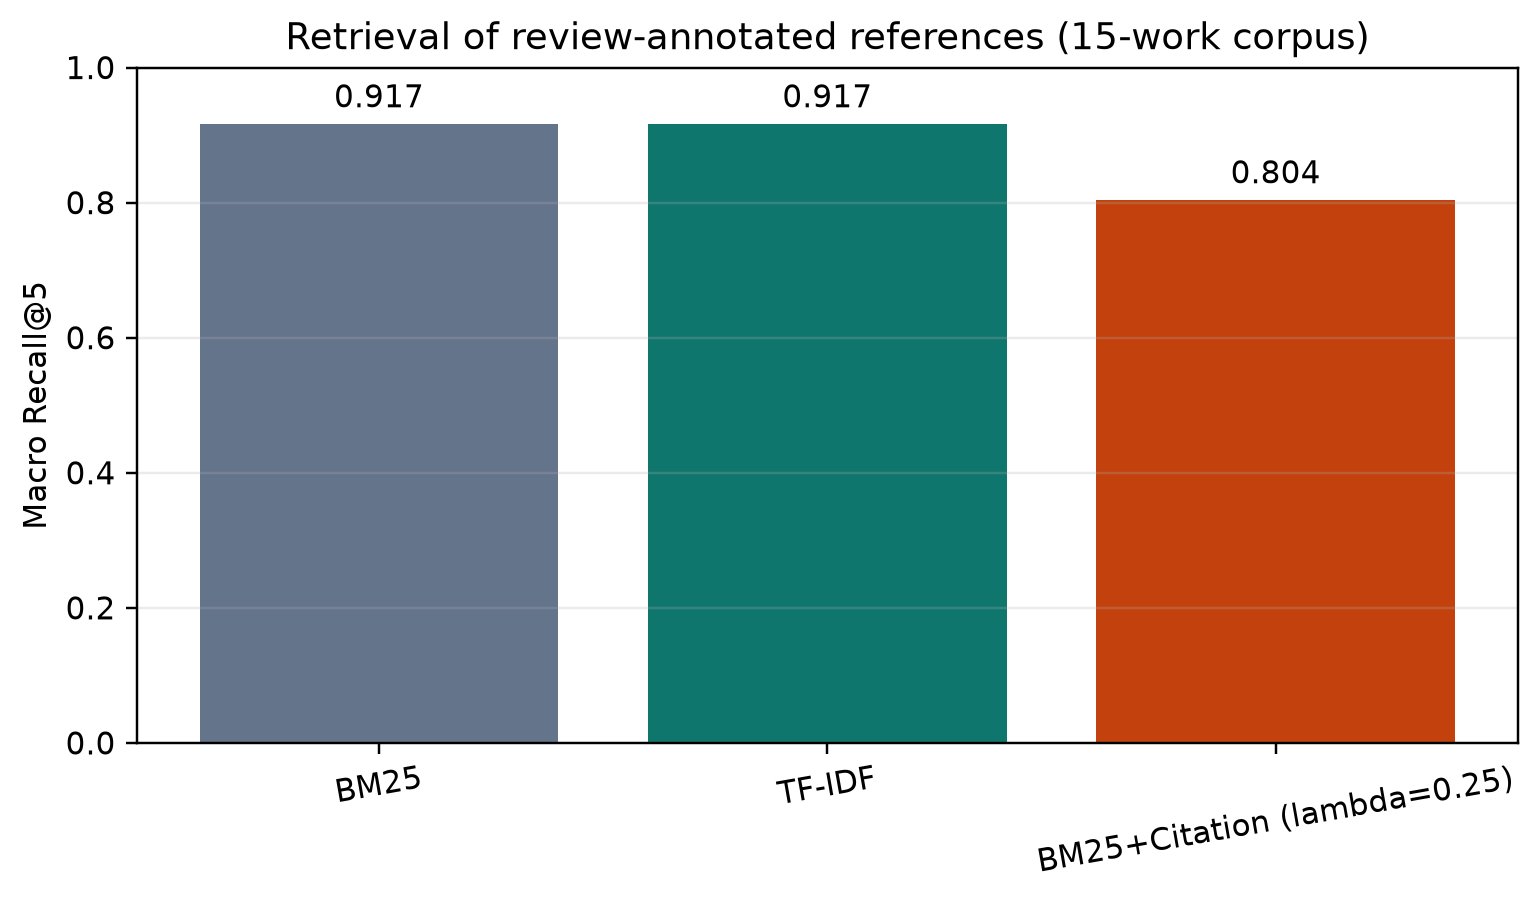
\includegraphics[width=.92\linewidth]{figures/recall_at_5.png}

\caption{Macro Recall@5 from the frozen ranking run. The citation prior reduces recall within the query-specific labels on this 15-work corpus.}

\end{figure}

The query-level pattern is not uniform. At lambda=0.25, Q1 remains at 2/3 relevant records in the top five, and Q4 retrieves all three of its relevant records under every method. The hybrid drops Q2 from 4/4 to 3/4 and Q3 from 5/5 to 4/5. The first relevant record remains at rank one for every query and method, which explains why mean reciprocal rank is 1.0 despite some relevant records leaving the top five.\par

\begin{table}[H]
\caption{Query-level Recall@5 by method.}
\centering\small
\begin{tabularx}{\linewidth}{XXXX}
\toprule
Query & BM25 & TF-IDF & BM25 + citation prior \\
\midrule
Q1 citation recommendation & 0.667 & 0.667 & 0.667 \\
Q2 language bias & 1.000 & 1.000 & 0.750 \\
Q3 LLM screening & 1.000 & 1.000 & 0.800 \\
Q4 retrieval and RAG & 1.000 & 1.000 & 1.000 \\
\bottomrule
\end{tabularx}
\end{table}

The changed top-five membership identifies two low-citation misses under the hybrid: R12 leaves Q2 and R04 leaves Q3. In each case, R10 enters the hybrid top five. R04 lacks an abstract in the frozen metadata, so its displacement can reflect both the citation prior and poorer lexical evidence. The experiment cannot isolate these causes for that record.\par

\section*{6 Sensitivity and interpretation}

The weight analysis in Table 4 and Figure 2 shows how the explicit prior changes the observed top-five set. At lambda=0.10, low-citation Recall@5 remains 1.000, while at lambda=0.25 and 0.50 it is 0.750. A pure citation ordering at lambda=1.0 reduces it to 0.000. Across these weights, mean log1p citations in the top five increases from 3.650 at lambda=0 to 8.305 at lambda=1.0. This is evidence of sensitivity to the prior strength on this corpus, not a recommended threshold for other systems.\par

\begin{table}[H]
\caption{Citation-prior weight sensitivity.}
\centering\small
\begin{tabularx}{\linewidth}{XXXX}
\toprule
lambda & Macro Recall@5 & Low-citation Recall@5 & Mean log1p cites, top 5 \\
\midrule
0.00 & 0.917 & 1.000 & 3.650 \\
0.10 & 0.917 & 1.000 & 4.249 \\
0.25 & 0.804 & 0.750 & 5.640 \\
0.50 & 0.804 & 0.750 & 6.418 \\
1.00 & 0.279 & 0.000 & 8.305 \\
\bottomrule
\end{tabularx}
\end{table}

\begin{figure}[H]

\centering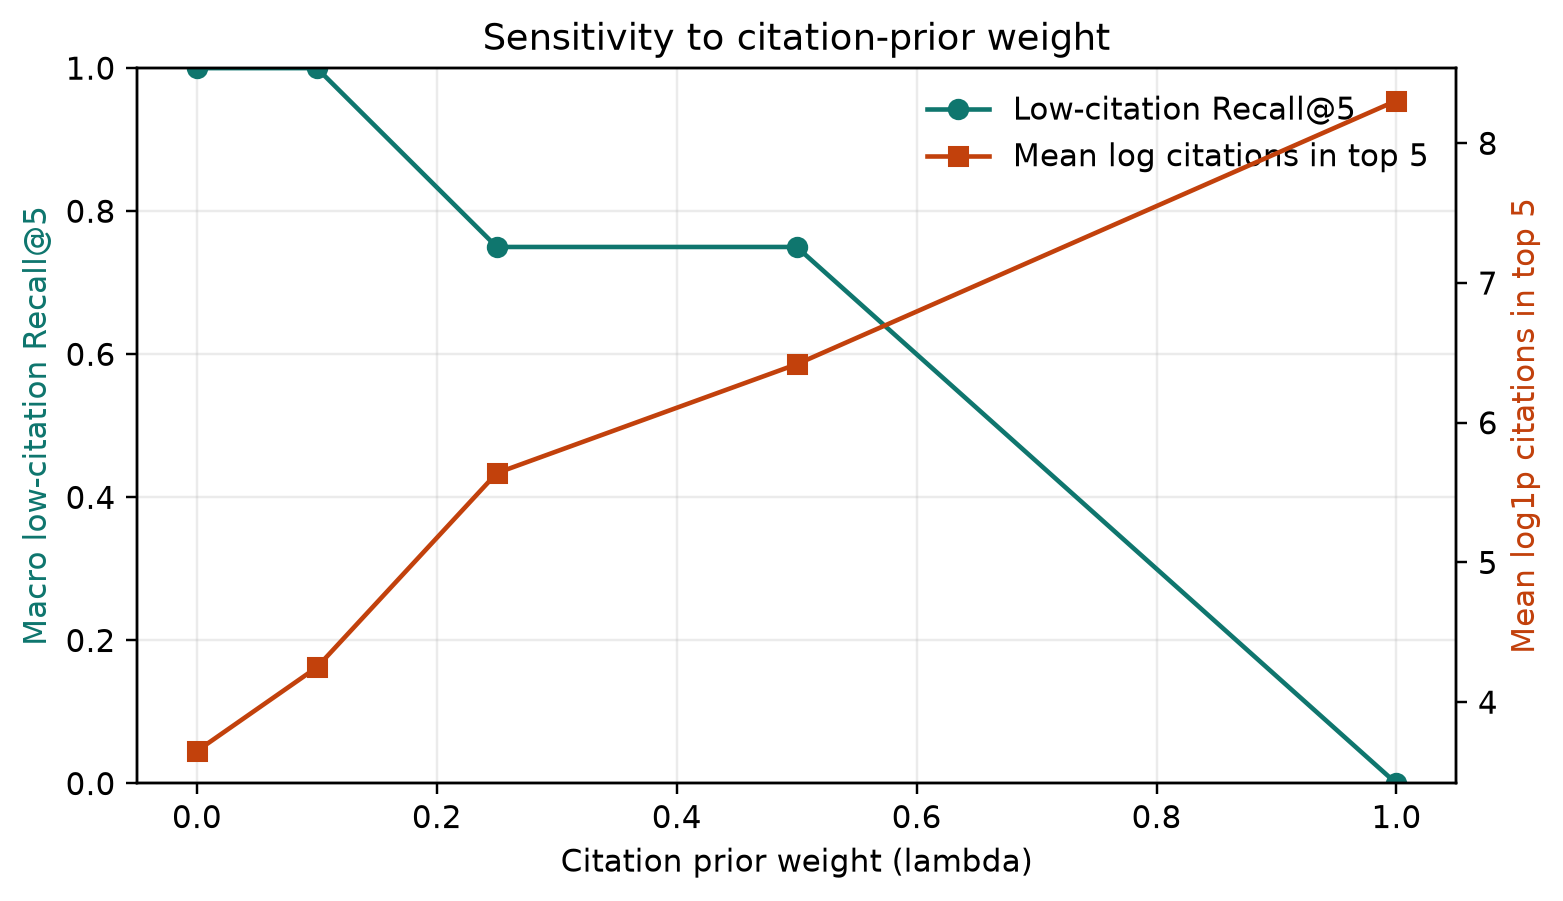
\includegraphics[width=.92\linewidth]{figures/citation_sensitivity.png}

\caption{As citation-prior weight rises, the top five contain higher-citation records; low-citation recall falls at weights of 0.25 and above in this run.}

\end{figure}

This pilot's result is mechanically connected to its intervention: the citation prior rewards high cited-by counts. The useful observation is not that citation-biased systems must always miss relevant papers, but that a modest explicit visibility feature displaced two records that the frozen review-derived labels mark as relevant. A broad source such as R10 is not necessarily useless to a human reviewer; the labels simply do not mark it as evidence for these two specific query sets. The metric reflects that protocol.\par

The experiment also illustrates why a single aggregate retrieval score can hide a subgroup change. Macro Recall@5 moves by 0.113 between BM25 and the primary hybrid, while low-citation recall moves by 0.250. These are descriptive differences on a small, constructed corpus. There is no estimate of uncertainty from independent query sampling, and the values should not be generalized to a scholarly search engine, a complete AI literature collection, or a parametric LLM recommender.\par

\section*{7 Threats to validity and limitations}

Construct validity is limited by the definition of relevance. Labels were created from one review's citations and explanatory text. They measure whether a source appears in the review's own evidence mapping, not whether it is relevant to every researcher or searcher using a similar query. A second independent reviewer and adjudication were not available.\par

External validity is very low by design. Fifteen cited works and four queries do not represent the full field. No works outside the bibliography can be retrieved, and the test cannot estimate end-to-end recall. Every indexed work is English-language metadata; the study does not compare English with non-English records or test the language-bias claims in the review.\par

Citation counts are confounded by publication age, field, venue, database coverage, and record-level versioning. R06 demonstrates the versioning issue directly: two OpenAlex records with the same title have different citation counts. The system pins one DOI record for reproducibility, but that count is not a canonical work-level count. The score also min-max normalizes citation counts over this tiny corpus, making the prior sensitive to its two extremely highly cited records.\par

The lexical baselines use abstracts when OpenAlex supplied them, but R04 is title-only. OpenAlex abstracts may be missing or indexed inconsistently. Queries are manually written and the relevance labels are derived from closely related review language, creating potential lexical overlap. The evaluation therefore measures ranking in a designed pilot setting and does not isolate a universal causal effect of citation metadata.\par

A stronger follow-up should form a candidate pool from a prespecified search across multiple bibliographic sources, include works not already cited by the review, establish double-screened labels, and freeze a test split before tuning. Citation exposure should be matched or normalized by publication year and field, and retrieval recall should be separated from title/abstract screening recall. A language-stratified benchmark would be needed to test language bias.\par

\section*{8 Reproducibility and responsible AI use}

The local project includes the frozen experiment configuration, corpus CSV, raw OpenAlex response snapshot, expanded relevance labels, source scripts, result CSVs, run metadata with SHA-256 hashes, and publication figures. The run uses Python 3.12.10 and matplotlib 3.11.2; the ranking functions use only the Python standard library. No GPU, API key, LLM, random seed, or training procedure is required. `python scripts/run\_experiment.py` regenerates the ranking and metric outputs from the included snapshot.\par

AI assistance was used to interpret the assignment, propose and implement this scoped experiment, and organize the manuscript and repository. The source checks, code execution, and actual outputs are recorded in the project decision, baseline validation, and AI assistance logs. The student should read and verify the implementation and sources before submission; AI-generated text or code is not independent authority.\par

\section*{9 Conclusion}

In a fixed corpus of 15 works cited by the supplied review, adding a normalized citation-count prior to BM25 at weight 0.25 increased the mean citation exposure of top-five results and reduced macro Recall@5 and low-citation Recall@5 relative to BM25 and TF-IDF. The sensitivity analysis shows that the size of this change depends on prior weight. The result answers a narrow implementation question and provides a runnable baseline, explicit protocol, and traceable output.\par

The experiment does not demonstrate field-wide recall bias, evaluate an LLM, or test language fairness. Its labels, candidate pool, citation counts, and query set limit the conclusions. The next defensible step is an independently annotated, broader candidate benchmark that tests visibility and language strata under a frozen retrieval protocol.\par

\bibliographystyle{ACM-Reference-Format}

\bibliography{references}

\end{document}
